\section{Trap problem and solution overview }
\label{sec:Trap problem and solution overview }

In this section, we first introduce the trap problem, and then given an overview of our solution.
\subsection{Trap problem}

As discussed earlier, APF-based heuristic algorithms may get caught into the "trap" problem. That is, when an AP is found, it may not be able to find a SRLG disjoint BP path even though a pair of disjoint paths do exist in the network.
%One typical way of solving the SRLG-disjoint routing problem is to have an Integer Linear Programming (ILP) formulation with the objective of jointly optimizing the selection of both AP and BP, and then find the solution for the problem through the branch-and-bound search. \note{"One typical way of solving the SRLG-disjoint routing problem" implies this is a very old problem.} With a high time complexity, the ILP-based algorithms are not feasible for large networks. To reduce the complexity, previous studies have shown that APF-based heuristics can achieve near-optimal solutions to the Min-Min SRLG-disjoint problem \note{This shows that this is not a new problem.} compared to their ILP-based counterparts \cite{xu2002ultra}.
%However, a solution based on the APF heuristic faces a big challenge. Once an AP is found, it may not be able to find a SRLG disjoint BP (even though a pair of disjoint paths do exist if a different AP is selected). This is the so-called {\em trap} problem.
%\note{You may not use "the" with short word. It does read well.}

Fig.\ref{fig:CompositeGraph}.(c),(d) illustrates the trap problem. The dotted line denotes an AP with its link set
$\mathbb{AP}=\{e_1,e_2,e_3$ $,e_4,e_5,e_6,e_7,e_8\}$. After removing the links on AP and also the links that share the common risks with AP, the remaining graph shown in Fig.\ref{fig:CompositeGraph}.(d) is obviously disconnected, so BP can not be found.

Although KSP is known as an effective algorithm to handle the trap
problem, it may face the problem of inefficiency.  Fig.\ref{fig:KSPproblem}  shows an example to illustrate why the KSP is extremely inefficient. In this graph, suppose  the link weights of $e_1, e_2, e_3, e_4$ are much larger than other links. Moreover, among $e_1, e_2, e_3, e_4$, the link weights of $e_1$ and $e_2$ are much smaller  than those of $e_3, e_4$. Then the first $K$ smallest weight paths from $s$ to $d$ found in the first $K$ tests will always contain the shortest path segment $e_1,e_2$ denoted by the dotted line. The first $K$ shortest APs will suffer from the trap problem, as $e_1$ and $e_4$ share the same risk and BP can not be found as a result. To avoid the trap problem, $K$ have to be set as a large value, which brings a high time complexity to KSP.

\begin{figure}[!h]
\centering
% Requires \usepackage{graphicx}
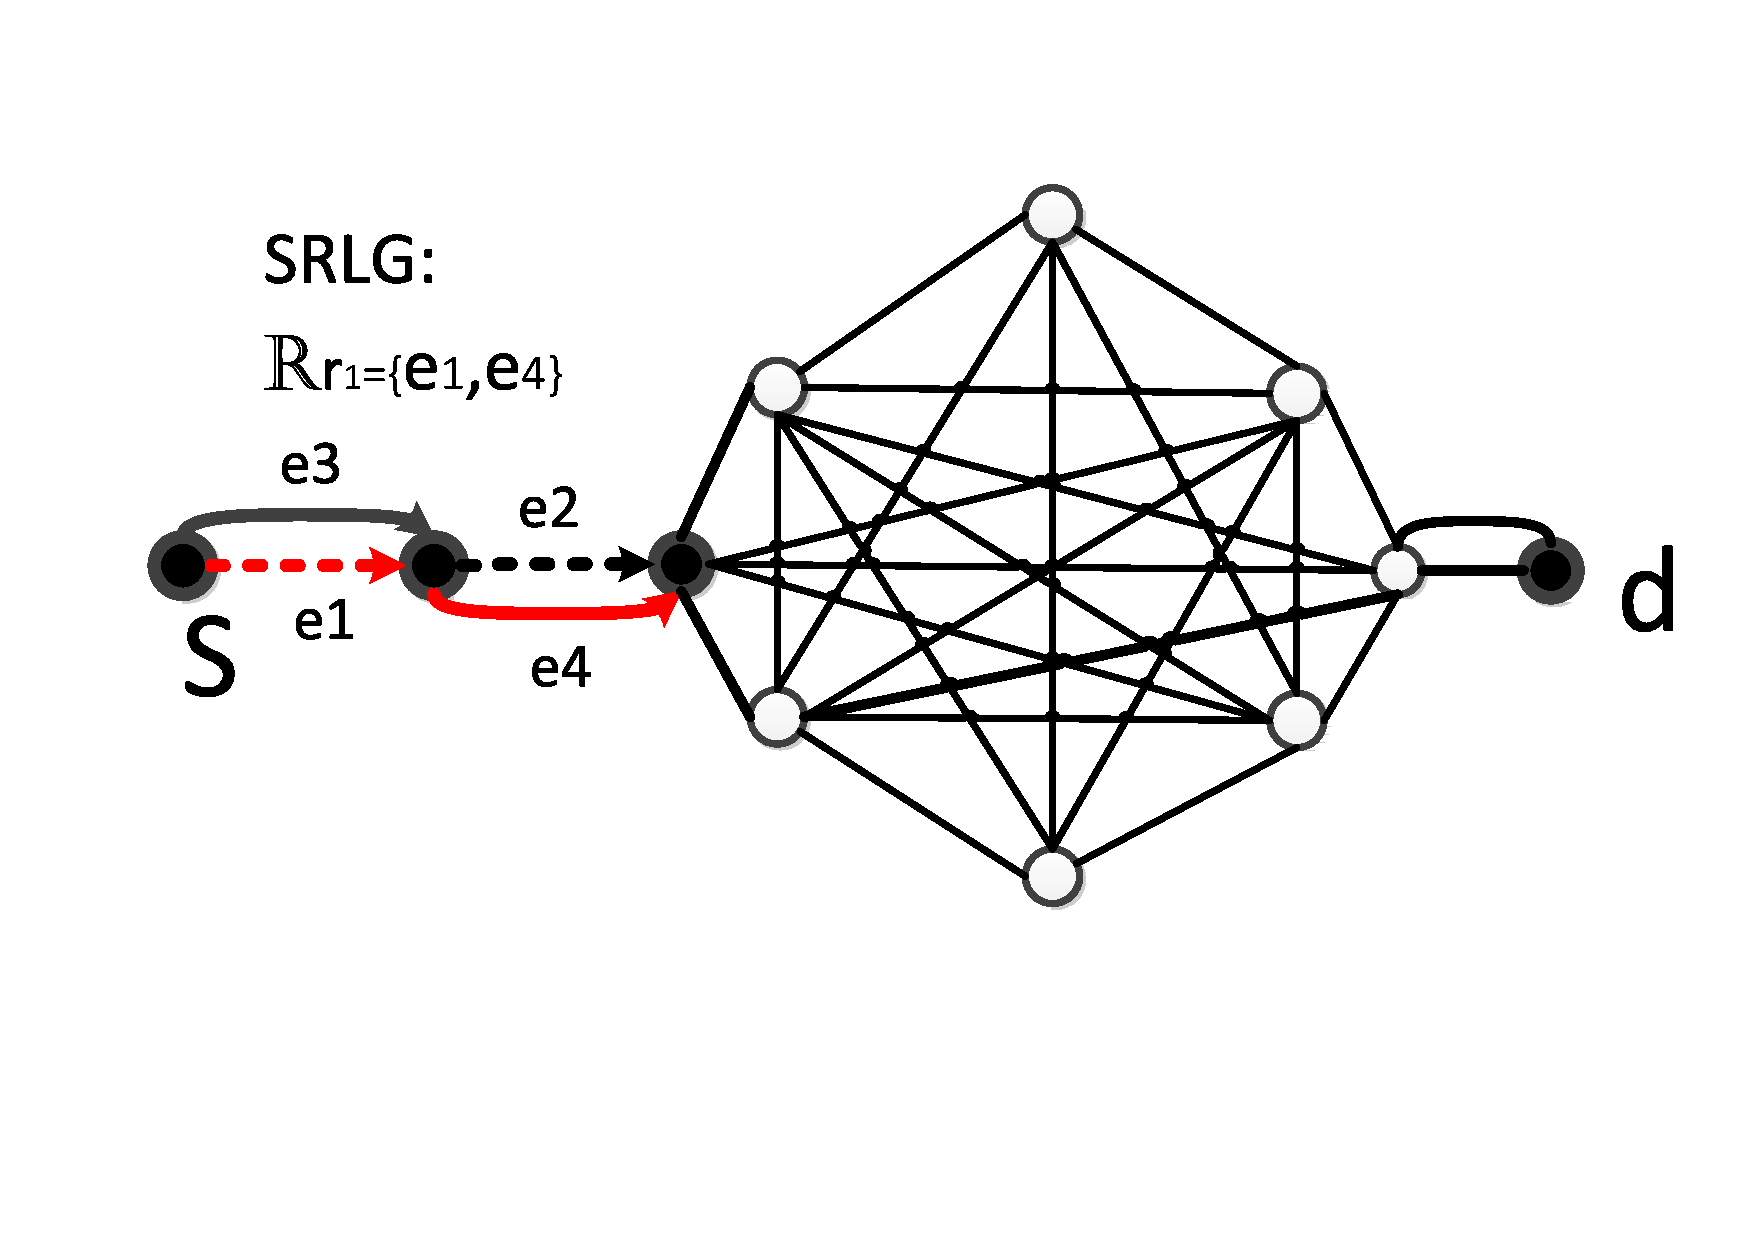
\includegraphics[width=2.8in]{franz/KSPproblem}
  \caption{An example to illustrate the inefficiency of KSP}
  \label{fig:KSPproblem}
\end{figure}

Given an AP that introduces the trap problem, the \textbf{SRLG Conflicting Link Set} is the sub-set of $\mathbb{AP}$ (where $\mathbb{AP}$ denotes the link set on this AP) so that no AP going through all these links in the sub-set can find a SRLG-disjoint BP. In Fig.\ref{fig:KSPproblem}, the AP that passes $e_1$ and $e_2$ \rev{introduces} the trap problem. \rev{The} SRLG Conflicting Link Set of this example is $\{e_1, e_2\}$.


%When a trap problem happens and there is no SRLG-disjoint BP can be found for a given AP, there may exist a sub-set of links in the $\mathbb{AP}$ such that no AP going through all these "problematic" links can find a SRLG-disjoint BP. In this paper, we call this set as a \textbf{SRLG Conflicting Link Set}.

Different from KSP,  when the shortest AP encounters the trap problem, we will address the issue through two major steps. We will first find the set of SRLG conflicting links  (Section \ref{sec:Find SRLG conflict link set}) like the set  $\{e_1,e_2\}$ in the example of Fig.\ref{fig:KSPproblem}, and then apply a divide and conquer algorithm (Section \ref{subsec:dividedconquer}) to partition the original problem into two sub-problems $\mathcal{P}(\emptyset,\{e_1\})$ and $\mathcal{P}(\{e_1\},\{e_2\})$. The two sub-problems can be executed in parallel on a multi-core CPU platform to quickly search for the SRLG disjoint path pair.
%\note{Such a long sentence. Can you still breathe? Also, why keep saying "firstly?" I could not understand why you can never change your writing problem.}

Although together all the links along the AP form such a SRLG Conflicting Link Set, we are interested in a set with as few links as possible. This is because the number of sub-problems to partition in our divide-and-conquer algorithm (in section \ref{subsec:dividedconquer}) is determined by  the size of the SRLG Conflicting Link Set. In Section \ref{subsec:Set cover problem for SRLG Conflicting Link Set}, we will present our solution to find the minimum SRLG Conflicting Link Set.


%For a given AP, we define its SRLG Conflicting Link Set to be a subset of the links on the AP \rev{path} such that no AP using all these "problematic" links can find a SRLG-disjoint BP. \note{Since this is found on an AP path, BP cannot be found for this AP, right? Also, why this set should be defined from an AP path?}  In Section \ref{subsec:Properties on the min-cut in the new graph $G^*$}, we will prove that a feasible SRLG Conflicting Link Set is a sub-set of the links on the AP. \note{Isn't it is a subset by your definition?: Why still need to probe it?}
%
%Although together all the links along the AP form such a SRLG Conflicting Link Set, \note{why?}

%(which impacts the algorithm's parallelism level)
%For the example in Fig.\ref{fig:Initial Graph}, \CI is $\{e_3,e_4,e_5,e_6\}$. Later, we will describe an algorithm to find \CI and prove that if any AP uses all the links in this \CI, no link-disjoint BP can be found. Note that, it is possible that an AP using all but one link in \CI can still have a BP.


\subsection{Divided-and-Conquer}
\label{subsec:dividedconquer}
After we obtain the SRLG Conflicting Link Set, we design a divide-and-conquer algorithm to partition the original Min-Min SRLG-disjoint routing problem into multiple sub-problems which can be executed in parallel to speed up the progress of SRLG disjoint path pair finding.

To facilitate the problem partition, we first define two disjoint link sets $\mathbb{I}$ and ${\mathbb{O}}$ with $\mathbb{I}\cap {\mathbb{O}}= \emptyset$,  where $\mathbb{I}$ is called the  inclusion set and ${\mathbb{O}}$ is called the exclusion set. Denoted by $\mathcal{P}({\mathbb{I},\mathbb{O}})$ the sub-problem (of the Min-Min SRLG-disjoint Problem) for finding a pair of AP and BP, where the AP is the shortest among all possible APs that $\textbf{must}$ use the links in $\mathbb{I}$ but $\textbf{not}$ use the links in ${\mathbb{O}}$.

Originally, let $\mathbb{I}=\emptyset$ and ${\mathbb{O}}=\emptyset$, the original Min-Min  SRLG-Disjoint Routing Problem can be represented by $\mathcal{P}(\emptyset,\emptyset)$. Note that, for any given link, the solution to $\mathcal{P}(\emptyset,\emptyset)$, if it exists at all, will use an AP that either contains the link or not. Given the SRLG Conflicting Link Set $\mathbb{T}$ with $|\mathbb{T}|$ links denoted by ${e_1},{e_2}, \cdots ,{e_{\left| \mathbb{T} \right|}}$, the original problem can be partitioned sequentially as follows.

Step 1, $\mathcal{P}(\emptyset,\emptyset)$ can be  divided into two sub-problems $\mathcal{P}(\emptyset,\{e_1\})$ and $\mathcal{P}(\{e_1\},\emptyset)$.

Step 2, similarly, $\mathcal{P}(\{e_1\},\emptyset)$ can be further divided into two sub-problems $\mathcal{P}(\{e_1,e_2\},\emptyset)$ and $\mathcal{P}(\{e_1\},\{e_2\})$.

The partition process continues until in the step $|\mathbb{T}|$, we have that $\mathcal{P}(\{e_1,e_2,\cdots ,{e_{\left| \mathbb{T} \right|-1}}\},\emptyset)$ can be further divided into two sub-problems $\mathcal{P}(\{e_1,e_2,\cdots ,{e_{\left| \mathbb{T} \right|-1}}, {e_{\left| \mathbb{T} \right|}}\},\emptyset)$ and $\mathcal{P}(\{e_1,e_2,\cdots ,{e_{\left| \mathbb{T} \right|-1}}\},\{e_{\left| \mathbb{T} \right|}\})$. Note that, as the sub-problem $\mathcal{P}(\{e_1,e_2,\cdots ,{e_{\left| \mathbb{T} \right|-1}}, {e_{\left| \mathbb{T} \right|}}\},\emptyset)$ has ${\mathbb{I}=\{e_1,e_2,\cdots ,{e_{\left| \mathbb{T} \right|-1}}, {e_{\left| \mathbb{T} \right|}}\}}$$=\mathbb{T}$ and ${\mathbb{O}}=\emptyset$, it has no solution.

We will try to find an optimal solution for each sub-problem except the sub-problem $\mathcal{P}(\{e_1,e_2,\cdots ,{e_{\left| \mathbb{T} \right|}}\},\emptyset)$, and then select the best one (i.e., the path pair with the shortest AP) to be the final (optimal) solution to the original problem $\mathcal{P}(\emptyset,\emptyset)$. If there is no solution to any of these sub-problems, we can guarantee that there is no solution to the original problem, as the way we divide the subproblems which has included  all possible disjoint path pairs.


In terms of the complexity, it should take less time to solve each sub-problem than the original problem itself as at least one link (which is from $\mathbb{T}$) will be removed from any further path computation for an AP, which also ensures that a different AP will be found and tested for the existence of a SRLG-disjoint BP.

When encountering the trap problem, our solution partitions the original problem and tests each sub-problem to look for the final solution. In our divide-and-conquer solution, the sub-problem is tested based on the SRLG Conflicting Link Set found from the AP encountering the trap problem. Compared to existing algorithms which search for alternative AP paths without considering the existing results and problems, our algorithm can largely reduce the computation cost.
%This  It is much more intelligent than other current technique in which when an AP encounter the trap problem, then test another AP that has no relationship with the previous AP. As the search direction is learned from previous AP,  our algorithm can largely reduce  computation cost.}
\begin{figure}[tp]
\small{
\begin{equation*}
{\mathcal P}(\emptyset ,\emptyset )\left\{ {\begin{array}{*{20}{l}}
{{\mathcal P}(\{ e_2\} ,\emptyset )\left\{ {\begin{array}{*{20}{l}}
{{\mathcal P}(\{ e_2,e_5\} ,\emptyset )\left\{ {\begin{array}{*{20}{l}}
{{\mathcal P}(\{ e_2,e_5,e_6\} ,\emptyset )}\\
{\boxed{{\mathcal P}(\{ e_2,e_5\} ,\{ e_6\} )}}
\end{array}} \right.}\\
{\boxed{{\mathcal P}(\{ e_2\} ,\{ e_5\} )}}
\end{array}} \right.}\\
{\boxed{{\mathcal P}(\emptyset ,\{ e_2\} )}}
\end{array}} \right.
\end{equation*}
}
\caption{Example to illustrate divide-and-conquer solution,$\mathbb{T}=\{e_2,e_5,e_6\}$.}
\label{fig:DividedConquer}
\end{figure}
For the example in Fig.\ref{fig:DividedConquer}, the SRLG Conflicting Link Set is $\mathbb{T}=\{e_2,e_5,e_6\}$.  The partition process can be shown in Fig.\ref{fig:DividedConquer}.  According to the SRLG Conflicting Link Set, we should try the total $3$ marked sub-problems ${{\mathcal{P}}(\{ e_2,e_5\} ,\{ e_6\} )}$, ${{\mathcal{P}}(\{ e_2\} ,\{ e_5\} )}$ and ${{\mathcal{P}}(\emptyset ,\{ e_2\} )}$,  and among which select the best one with the lowest AP path weight to be the final (optimal) solution to the original problem  $\mathcal{P}(\emptyset,\emptyset)$.


Note that we do not need to solve the sub-problems ${{\mathcal{P}}(\{ e_2,e_5\}, \emptyset)}$ and ${{\mathcal{P}}(\{ e_2\},\emptyset )}$, as their solutions have already been included in the sub-problems above. The solution space of the first one consists of two sub-problems ${{\mathcal P}(\{ e_2,e_5,e_6\} ,\emptyset )}$ and ${{\mathcal P}(\{ e_2,e_5\} ,\{ e_6\} )}$. As the  SRLG Conflicting Link Set is $\mathbb{T}=\{e_2,e_5,e_6\}$, obviously, the sub-problem ${{\mathcal P}(\{ e_2,e_5,e_6\} ,\emptyset )}$ does not have a solution. Thus the solution space of  ${{\mathcal P}(\{ e_2,e_5\} ,\{ e_6\} )}$ is equal to that of ${{\mathcal{P}}(\{ e_2, e_5\}, \emptyset)}$.  Similarly, the solution space of ${{\mathcal{P}}(\{ e_2\},\emptyset )}$ includes that of ${{\mathcal{P}}(\{ e_2\} \{ e_5\}, \emptyset)}$  and ${{\mathcal{P}}(\{ e_2\} ,\{ e_5\} )}$.



When a trap problem happens, the number of sub-problems to test is $|\mathbb{T}|$, which is equal to the size of the SRLG Conflicting Link Set. To reduce the complexity, in Section \ref{subsec:Set cover problem for SRLG Conflicting Link Set}, we focus on finding the minimum SRLG Conflicting Link Set given an AP.
